% arara: xelatex
% arara: xelatex
% arara: xelatex


% options:
% thesis=B bachelor's thesis
% thesis=M master's thesis
% czech thesis in Czech language
% english thesis in English language
% hidelinks remove colour boxes around hyperlinks

\documentclass[thesis=M,english]{FITthesis}[2023/2/2]

%\usepackage[utf8]{inputenc} % LaTeX source encoded as UTF-8
% \usepackage[latin2]{inputenc} % LaTeX source encoded as ISO-8859-2
% \usepackage[cp1250]{inputenc} % LaTeX source encoded as Windows-1250

% \usepackage{subfig} %subfigures
% \usepackage{amsmath} %advanced maths
% \usepackage{amssymb} %additional math symbols

\usepackage{dirtree} %directory tree visualisation
\usepackage{xcolor}
\usepackage{xspace}
\usepackage{amsmath}
\usepackage{amssymb}
\usepackage{graphicx}
\usepackage{subfig}
\usepackage{float}
\usepackage{nameref}
\usepackage{algorithm}
\usepackage{algpseudocode}
\usepackage{pdfpages}

\graphicspath{ {./assets/} }
% % list of acronyms
% \usepackage[acronym,nonumberlist,toc,numberedsection=autolabel]{glossaries}
% \iflanguage{czech}{\renewcommand*{\acronymname}{Seznam pou{\v z}it{\' y}ch zkratek}}{}
% \makeglossaries

% % % % % % % % % % % % % % % % % % % % % % % % % % % % % % 
% EDIT THIS
% % % % % % % % % % % % % % % % % % % % % % % % % % % % % % 

\department{Department of Applied Mathematics}
\title{Material Picker: tool for detecting material properties}
\authorGN{Viet Anh} %author's given name/names
\authorFN{Tran} %author's surname
\author{Viet Anh Tran} %author's name without academic degrees
\authorWithDegrees{Bc. Viet Anh Tran} %author's name with academic degrees
\supervisor{Ing. Tomáš Nováček}

\acknowledgements{me, myself and I}


\abstractEN{TODO
}

\abstractCS{TODO CZ}
\placeForDeclarationOfAuthenticity{Prague}
\keywordsCS{TODO}
\keywordsEN{TODO}
\declarationOfAuthenticityOption{1} %select as appropriate, according to the desired license (integer 1-6)
% \website{http://site.example/thesis} %optional thesis URL


%========================================================================================================
\begin{document}
%========================================================================================================
	%========================================================================================================
	\setsecnumdepth{part}
	\chapter{Introduction}\label{ch:introduction}
	Computer graphics and 3D modeling is a fundamental field in our constantly increasing digital world. Its application in engineering, science, art, product visualization, and most notably, entertainment has pushed this field with a constant demand for better visual quality and performance optimization.

3D models create the very core of any 3D visualization, bringing objects to computer-generated 3D space. The 3D model defines the shape of an object and can be further improved to closely represent real-world objects by applying textures, lighting, and many more techniques. Models are typically created in 3D modeling software by an artist or by 3D scanning. 3D scanning can often bring too many details in terms of polygon numbers. A shape that could be perfectly recognizable by ten polygons would now be described by thousands. The side effect of things is big hardware requirements.

Lowering the number of polygons is a usual practice done either manually or by many developed tools over the years. These tools do not consider any edge flow, a critical feature particularly important for character modeling and animation. Edge flow allows smooth deformation. In terms of animation, we can look at muscle movement, optimal edge avoids wrinkled defects on the character model, and the skin would stretch and contract in a way as we are used to seeing in the real world.

This thesis aims to introduce the final step in polygon reduction workflow when using tools. We present a neural network taking a 3D model and outputting an improved model in terms of edge flow quality, approximating similar polygon quantity.

\begin{description}

    \item In Chapter \nameref{ch:neural_network}, we explore basics of neural networks, introduce its terminology and several commonly used network architectures.
    
    \item In Chapter \nameref{ch:implementation}, we describe used methods and key implementation points of our work.
    
    \item In Chapter \nameref{ch:experiments}

    \item In \nameref{ch:conclusion}, we evaluate the results of the work and suggest possible improvements for future works.
\end{description}\newpage\cleardoublepage
	%========================================================================================================
	\setsecnumdepth{all}
	\chapter{Neural Networks}\label{ch:neural_network}
	An artificial neural network (ANN), first introduced by Warren McCulloch and Walter Pitts in "A logical calculus of the ideas immanent in nervous activity" published in 1943 \cite{mcculloch1943logical}, is a mathematical model based on biological neural networks. It 
carries the ability to learn and correct errors from previous experience \cite{designimplentationcc}, \cite{bengio2017deep}.

The ANN has gained popularity in recent years with still increasing advancements in technology and availability of training data. ANN now becomes a default solutions for complex tasks previously thought to be unsolvable by computers \cite{neural2016krishtopa}.

This chapter will briefly introduce different types of neural units and their activation functions, along with some commonly used network architectures.

\setsecnumdepth{all}
\section{Artificial Neuron}
Artificial neurons are units of ANN, mimicking behavior of biological neurons. Just as biological neurons, it can receive as well as pass information to other neurons.

\setsecnumdepth{all}
\subsection{Perceptron}
Perceptron, developed by Frank Rosenblatt in 1958 \cite{perceptronprobabmodel}, is the simplest class of artificial neurons.

Perceptron takes several binary inputs in form of a vector $\vec{x} = (x_1, x_2,...,x_n)$, and outputs a single binary number. Perceptron uses real numbers called \textit{weights}, assigned to each edge, vector $\vec{w} = (w_1,w_2,...,w_n)$, to express the importance of respected input edges, 

A \textit{step function} calculates the perceptron's output.
The function output is either 0 or 1 determined by whether its weighted sum $\alpha = \sum_{i} x_i w_i$ is less or greater than its \textit{threshold} value, a real number, usually represented as an incoming edge with a negative weight -1 \cite{matous}.

\begin{equation}
    output =
\begin{cases}
    1, & \text{if $\alpha\ \geq\ threshold$}\\
    0, & \text{if $\alpha\ <\ threshold$}
\end{cases} 
\end{equation} 


\begin{figure}[h]
	\centering
    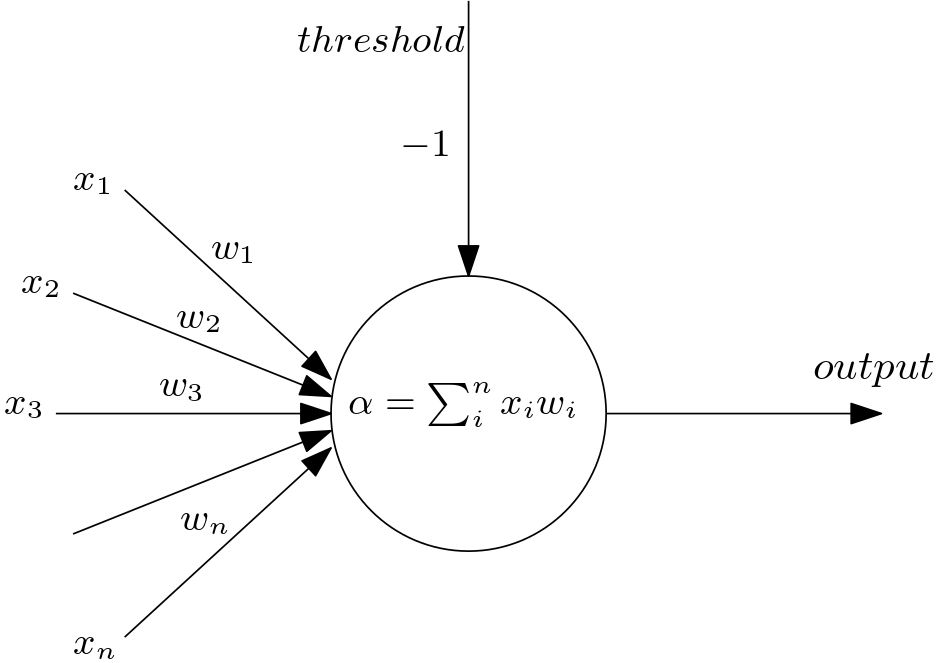
\includegraphics[width=12cm]{perceptron.png}
	\caption{Perceptron \cite{matous}}
	\label{fig:perceptron}
\end{figure}

%=======================================================================================================================
\subsection{Sigmoid Neuron}
Sigmoid neuron, similarly to perceptron, has vector inputs $\vec{x}$ and weights. The difference is in the output value and its calculation. Instead of perceptron's binary output 0 or 1, a sigmoid neuron outputs a real number between 0 and 1 using a \textit{sigmoid function} \cite{nndl2015michaelnielsen}, \cite{rojas2013neural}, \cite{matous}.

\begin{equation}
    {\sigma(\alpha) = \frac{1}{1 + e^{-\alpha}}}
\end{equation}

\begin{figure}[h]
	\centering
    \subfloat[\centering Step function]{{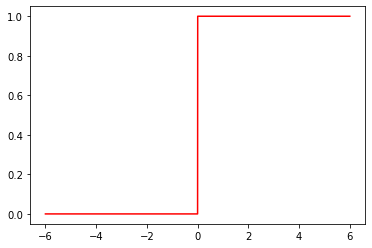
\includegraphics[width=6cm]{step}}\label{step_function}}%
    \qquad
    \subfloat[\centering Sigmoid function]{{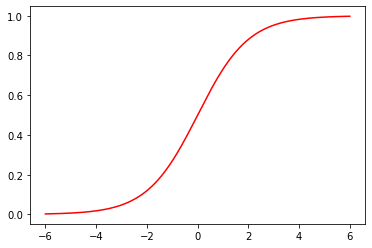
\includegraphics[width=6cm]{sigmoid}}\label{sigmoid_function}}%
    \caption{Comparison between step function and sigmoid function}
    \label{sigmoid_neuron}
\end{figure}
As shown in Figure \ref{sigmoid_neuron}, the sigmoid function (\ref{sigmoid_function}) is a smoothed-out  step function (\ref{step_function}).

%=======================================================================================================================
\subsection{Activation Function}
An artificial neuron's activation function defines neuron's output value for given inputs, commonly being ${f: \mathbb{R} \rightarrow \mathbb{R}}$ \cite{leskovec2020mining}. An important trait of many activation functions is their differentiability, allowing them to be used for \textit{Backpropagation}, ANN training algorithm. The activation function needs to have a derivative that does not saturate when headed towards 0 or explode when headed towards inf \cite{matous}.

For such reasons, step function or any linear function are unsuitable for ANN.
% Sigmoid Function ==========================================================================================================
\setsecnumdepth{all}
\subsubsection{Sigmoid Function}
The sigmoid function is often used in ANN as an alternative to the step function. A popular choice of the sigmoid function is a \textit{logistic sigmoid}, output value ranging between 0 and 1.

\begin{equation}
    {\sigma(\alpha) = \frac{1}{1 + e^{-\alpha}} = \frac{e^x}{1 + e^{x}}}
\end{equation}


% \begin{figure}[h]
%   \centering
%     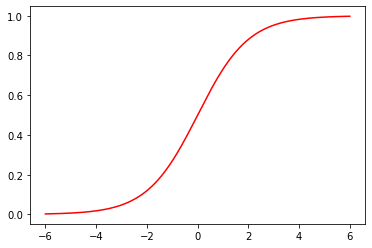
\includegraphics[width=7cm]{sigmoid}
%   \caption{Sigmoid function}
%   \label{fig:sigmoid}
% \end{figure}


One of the reasons for its popularity is the simplicity of its derivative calculation:

\begin{equation}
    {\frac{d}{dx}\sigma(\alpha) = \frac{e^x}{(1 + e^{x})^2} = \sigma(x)(1-\sigma(x))}
\end{equation}


Its disadvantages is the \textit{vanishing gradient}. A problem where if given a very high or very low input values, the prediction would stay almost the same. Possibly resulting in training complications or performance issues \cite{7typesactivationfunctions}, \cite{matous}.

% Hyperbolic Tangent ==========================================================================================================

\subsubsection{Hyperbolic Tangent}

Hyperbolic tangent is similar to logistic sigmoid function with a key difference in its output, ranging between -1 and 1.

\begin{equation}
    {tanh(x) = \frac{e^x - e^{-x}}{e^x + e^{-x}}}
\end{equation}


\begin{figure}[h]
    \centering
    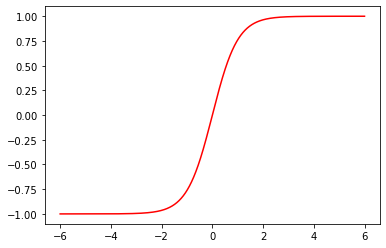
\includegraphics[width=8cm]{tangent}
    \caption{Hyperbolic tangent \cite{matous}}
    \label{fig:hyperbolictangent}
\end{figure}


It shares the sigmoid's simple calculation of its derivative.

\begin{equation}
    {\frac{d}{dx}\tanh(x) = 1 - \frac{(e^x - e^{-x})^2}{(e^x + e^{-x})^2} = 1 -\tanh^2(x)}
\end{equation}

By being only moved and scaled version of the sigmoid function, hyperbolic tangent shares not only sigmoid's advantages but also its disadvantages \cite{leskovec2020mining}, \cite{matous}.

% Rectified Linear Unit ==========================================================================================================

\subsubsection{Rectified Linear Unit}

The output of the Rectified Linear Unit (ReLU) is defined as:

\begin{equation}
    f(x) = max(0,x)
\begin{cases}
    x, & \text{if $x\ \geq\ 0$}\\
    0, & \text{if $x\ <\ 0$}
\end{cases} 
\end{equation} 

\begin{figure}[h]
    \centering
    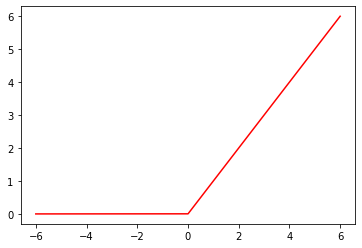
\includegraphics[width=7cm]{relu}
    \caption{Rectified Linear Unit \cite{matous}}
    \label{fig:relu}
\end{figure}


ReLU's popularity is mainly due to its computational efficiency \cite{7typesactivationfunctions}. Its disadvantages begin to show themselves once inputs approach zero or to a negative number. Causing the so-called dying ReLu issue, where the network is unable to learn anymore. There are many variations of ReLu to this date, e.g., Leaky ReLU, Parametric ReLU, ELU, ...
% Softmax ==========================================================================================================

\subsubsection{Softmax}

Softmax separates itself from all the previously mentioned functions by its ability to handle multiple input values in the form of a vector $\vec{x} = (x_1,x_2,...,x_n)$ and output for each $x_i$ defined as:

\begin{equation}
    {\sigma(x_i) = \frac{e^x_i}{\sum_{j=1}^{n}e^x_j}}
\end{equation}

Output is normalized probability distribution, ensuring $\sum_{i}\sigma(x_i) = 1$ \cite{lipton2015critical}. It is being used as the last activation function of ANN, normalizing the network's output into $n$ probability groups.

%=======================================================================================================================
%=======================================================================================================================
\section{Types of Neural Networks}

To this day, there are many types and variations of ANN, each with its structure and use cases. Here we will briefly introduce the most common ones, such as feed-forward networks, convolutional neural networks, or recurrent neural networks.

\setsecnumdepth{all}
\subsection{Feed-forward Networks}
Feed-forward network (FFN), the first invented ANN and the simplest variation of an ANN. Its name comes from the way how information flows through the network. The data flows in one direction, oriented from the \textit{input layer} to the \textit{output layer}, without cycles. The input layer takes input data, vector $\vec{x}$, producing $\hat{y}$ at the output layer \cite{ffnbrilliant}.

FFN contains several hidden layers of various widths but it can also have no hidden layers at all. By having no back-loops, FFN generally minimizes error, computed by \textit{cost function}, in its prediction by using the \textit{backpropagation} algorithm to update its weight values \cite{mainTypesANN}, \cite{lipton2015critical}.

\begin{figure}[h]
    \centering
    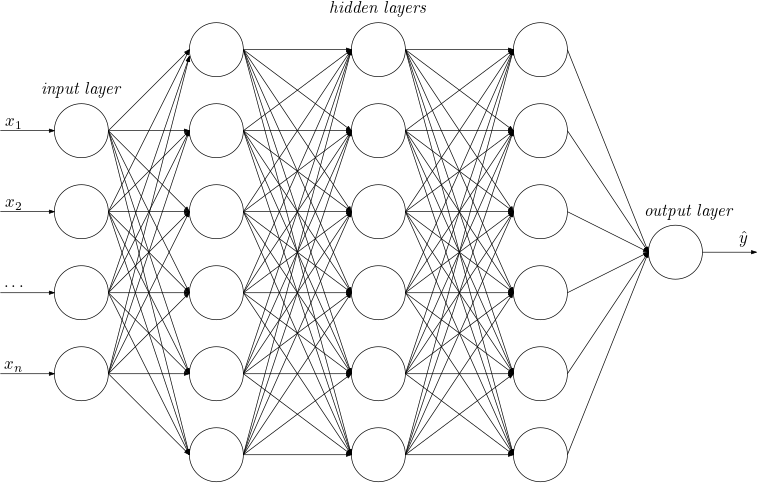
\includegraphics[width=12cm]{ffn.png}
    \caption{Fully connected Feed-forward Neural Network \cite{matous}}
    \label{fig:ffn}
\end{figure}

%=======================================================================================================================

\subsubsection{Cost Function}
Cost function $C(\vec{w})$ is used in ANN's training process. It takes all weights and biases of an ANN as its input, in the form of a vector $\vec{w}$ and calculates a single real number expressing ANN's error in prediction \cite{Goodfellow-et-al-2016}. Higher number expressing poor prediction and as the number gets lower the ANN's output gets closer to the correct result. The main goal of training is to minimize the cost function. 

%=======================================================================================================================
\subsubsection{Backpropagation}
Backpropagation, short of backward propagation of errors, is a widely used algorithm in training FFN using \textit{gradient descent} to find a local minimum of a cost function and update ANN's weights \cite{birlliantbackprop}.

The gradient of a multi-variable function provides us with the direction of the gradient ascent, where we should step to rapidly increase the output and find the local maximum. Conversely, the negative of the gradient points towards the local minimum.'

It is common practice to split training samples into small \textit{batches} of size $n$. For each sample in the batch, we will calculate a gradient descent and use their average gradient descent to update the network's weights. This average gradient descent indicates the adjustments that need to be made to the weights so that the artificial neural network (ANN) moves closer to the correct results \cite{birlliantbackprop}.

\begin{equation}
    {- \gamma \nabla C(\vec{w}_i) + \vec{w}_i \rightarrow \vec{w}_{i+1} }
\end{equation}

$\vec{w_i}$ is weights of the network at the current state (batch), $\vec{w_{i+1}}$ is updated weights, $\gamma$ is the learning rate and $-\nabla C(\vec{w_i})$ is the gradient descent.

%=======================================================================================================================
\subsection{Convolutional Neural Networks}
The primary objective of a Convolutional Neural Network (CNN) is to enable a computer to identify images and objects, making it ideal for image classification and object recognition tasks. 

CNNs are based on the biological processes in the human brain and its connectivity patterns resemble those of the human visual cortex. However, images are perceived differently by the human brain and a computer, with the latter interpreting images as arrays of numbers. As a result, CNNs are designed to work with two-dimensional image arrays, although they can also work with one-dimensional or three-dimensional arrays \cite{mlmastery}.

CNN is a variation of FNN \cite{Goodfellow-et-al-2016}.  It typically consists of an input layer, followed by multiple hidden layers, including several \textit{convolutional layers} and \textit{pooling layers}, and concluding with an output layer.

\setsecnumdepth{all}
\subsubsection{Convolutional Layer}

The convolutional layer's goal is to extract key features from the input image by passing a matrix known as a \textit{kernel} over the input image abstracted into a matrix \cite{mathworkscnn}.

\begin{figure}[h]
	\centering
    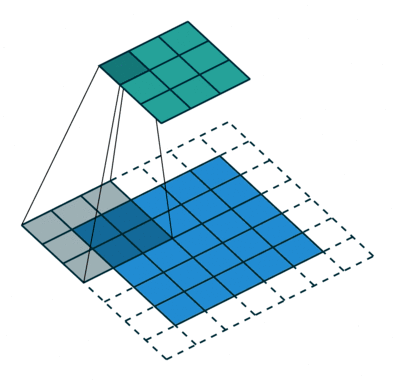
\includegraphics[width=8cm]{conv_layer_padding.png}
	\caption{Convolution of an 5x5x1 image with 3x3x1 kernel \cite{compguideCnn}}
	\label{fig:cnn_conv}
\end{figure}


The outcome of a convolution operation can be either reduced or increased in size. If the size is reduced, it is referred to as \textit{valid padding}. For example, a convolution operation on an 8x8 input image would result in a 6x6 convoluted feature. On the other hand, if the size remains the same or is increased, it is referred to as \textit{same padding} \cite{compguideCnn}.

\subsubsection{Pooling Layer}


Like the convolutional layer, the pooling layer reduces the size of the convolved feature to reduce computational power needed for data processing. It also extracts dominant features that are invariant to rotation and position, making it beneficial for training the model effectively \cite{compguideCnn}.

There are two types of pooling: max pooling and average pooling. Max pooling returns the maximum value from the portion of the image covered by the kernel, acting as a noise suppressant by removing noisy activations and performing de-noising and dimensionality reduction. Average pooling returns the average of all values in the same portion, reducing dimensions as a noise suppression mechanism. It is worth noting that max pooling performs better \cite{compguideCnn}.

\begin{figure}[h]
	\centering
    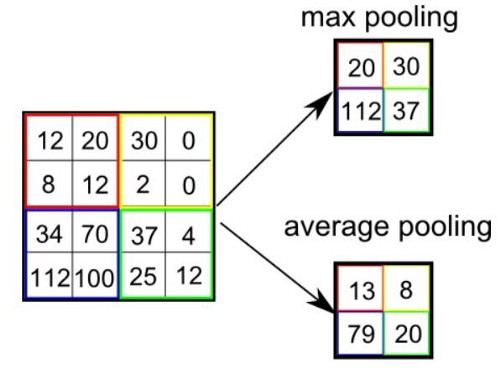
\includegraphics[width=8cm]{conv_pooling.png}
	\caption{Types of pooling \cite{compguideCnn}}
	\label{fig:cnn_pooling}
\end{figure}

%=======================================================================================================================
%\subsection{Recurrent Neural Networks}
%Recurrent Neural Network (RNN) is distinguished by its memory, which can handle input sequences of any length. Its past predictions influence influence the current output. Resulting in different predictions depending on previous inputs in the sequence \cite{rnnDSmedium}.

RNNs are widely used in fields like speech recognition, image captioning, natural language processing, and language translation and are found in popular applications such as Siri, Google Translate, and Google Voice search \cite{ibmrnn}.

To illustrate how RNNs use previous inputs, consider the idiom "feeling under the weather." To understand the meaning, the words must be in a specific order. RNNs take into account the order of the words and use the information from each word to predict the next word in the sequence. Each time step represents a single word, so for example, the third time step represents "the." The hidden state of the RNN holds information from previous inputs, such as "feeling" and "under" \cite{ibmrnn}.

\begin{figure}[h]
    \centering
    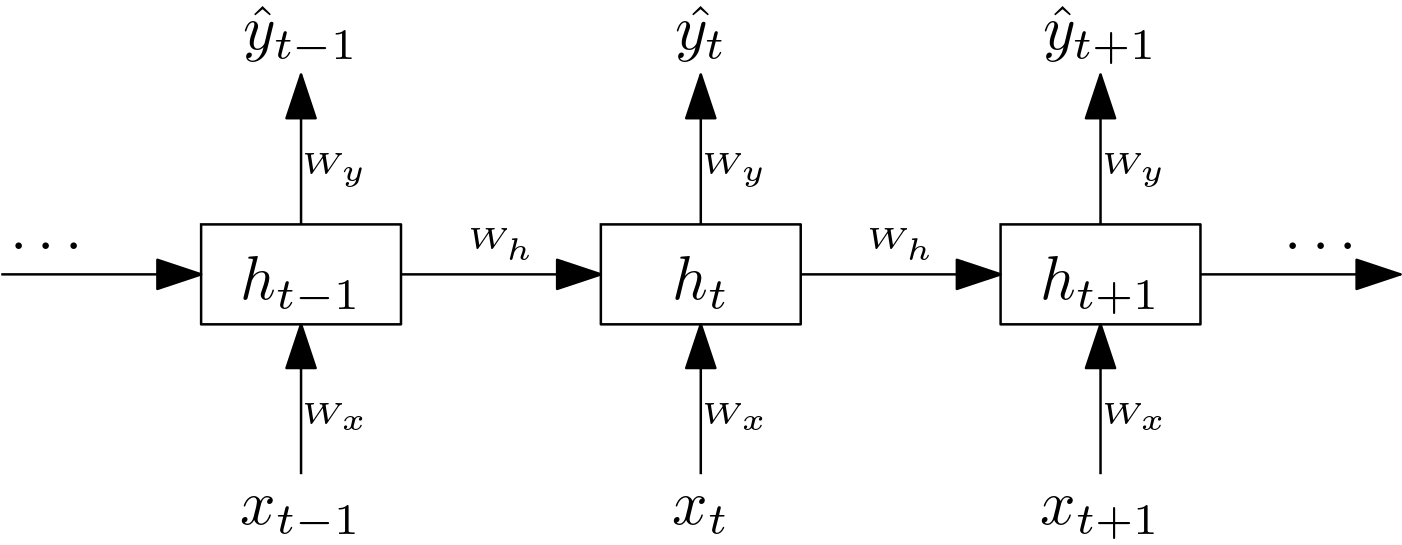
\includegraphics[width=12cm]{rnn_u.png}
    \caption{Unrolled structure of RNN \cite{matous}}
    \label{fig:rnn}
\end{figure}


Figure \ref{fig:rnn} depicts how the RNN network operates at each time step $t$. The current input $\vec{x_t}$ is processed by the network to produce the output $\hat{y}_t$, the next timestep of the input is $x_{t+1}$ with additional input from the previous time step from the hidden state $h_{t}$. This allows the neural network to have a context from previous inputs while processing the current input. The ability to hold past values and work with a context in the data is due to the recurrent units, reffered to as memory \cite{rnnin6}.

The recurrent unit is calculated as follows:

\begin{equation}
    {h_t = f(W_{x}x_t + W_{h}h_{t-1}+\vec{b_h})}
\end{equation}

$f$ is the activation function, $W_x,W_h$ are weight matrixes, $x_t$ is the input, and $\vec{b_h}$ is the vector of bias parameters. The hiddent stat $h_t$ at time step $t=0$ is initialized to $(0,0,...,0)$. The output $\hat{y_t}$ is then calculated as:

\begin{equation}
    {\hat{y}_t = g(W_{y}h_t + \vec{b_y})}
\end{equation}

$g$ is also an activation function, typically softmax, ensuring the output is in the desired class range. $W_y$ is the weight matrix, and $\vec{b_y}$ is a vector of biases determined during the learning process.

Training RNNs uses a modified version of the backpropagation algorithm called \textit{backpropagation through time} (BPTT). This process works by unrolling the RNN \cite{Goodfellow-et-al-2016}, computing the losses across each time step, and then using the backpropagation algorithm to update the weights. More on RNN in \cite{lipton2015critical} by Lipton et al.


%=======================================================================================================================
%\subsection{Long Short-Term Memory}
%Consider a task where we attempt to predict the last word in a sentence "The clouds are in the \textit{sky}". It is fairly obvious the last word is meant to be "\textit{sky}". The gap between the relevant information and the prediction place is small, RNNs can learn to use past information and make accurate predictions. However, if we consider "I grew up in Spain... I speak fluent \textit{Spanish}", the gap between the relevant information and predicting word is large. As the gap grows, RNNs are unable to handle the task. Such problem is called \textit{long-term dependencies} \cite{colahLSTM}.

Long Short Term Memory networks (LSTM), first introduced by Hochreiter S. and Schmidhuber J. \cite{hochreiterLSTM}, are RNN architecture with the ability to handle long-term dependencies. LSTMs replace RNN's hidden states with \textbf{LSTM Cells} and add connections between cells, known as \textit{cell states} or $c_{t}$. Each LSTM Cell consists of three gates that regulate the input and output of the cell and its calculation runs as follows:

1. \textbf{Forget Gate}: Controls which information to keep and which to discard. \textit{Sigmoid function} produces a value ranging from 0 to 1 base on the information from the previous hidden state and from the current input. The value closer to 0 indicates that the information should be discarded, while a value closer to 1 means it should be kept.

\begin{equation}
    {f_t = \sigma(W_{x_f}x_t + W_{h_f}h_{t-1}+\vec{b_f})}
\end{equation}

2. \textbf{Input Gate}: Decides which information should be updated. The sigmoid function a value between 0 and 1 based on the previous hidden state and the current input state. A value close to 0 indicates unimportant information, while a value close to 1 indicates important information.

\begin{equation}
    {i_t = \sigma(W_{x_i}x_t + W_{h_i}h_{t-1}+\vec{b_i})}
\end{equation}

The information from the previous hidden state and the current input state are processed by a \textit{tanh} function, which results in values ranging from -1 to 1.

\begin{equation}
    {g_t = \tanh(W_{x_g}x_t + W_{h_g}h_{t-1}+\vec{b_g})}
\end{equation}

The decision on how to update the cell is obtained by multiplying sigmoid output and $\tanh$ output. With all the required values available, we can now calculate the \textit{cell state} as follows:

\begin{equation}
    {c_t = i_t \odot g_t + f_t \odot c_{t-1}}
\end{equation}


3. \textbf{Output Gate}: Determines what information should the next hidden state contain. The previous hidden state and the current input are passed into a sigmoid function.

\begin{equation}
    {o_t = \sigma(W_{x_o}x_t + W_{h_o}h_{t-1}+\vec{b_o})}
\end{equation}

Passing the newly modified cell state into a tanh function and multiplying its output with the sigmoid output, we get the hidden state \cite{guideLSTM}.

\begin{equation}
    {h_t = o_t \odot tanh(c_t)}
\end{equation}


The output $\hat{y}_t$ is calculated the same way as regular RNN \cite{matous}.

\begin{equation}
    {\hat{y}_t = g(W_{y}h_t + \vec{b_y})}
\end{equation}

\begin{figure}[h]
    \centering
    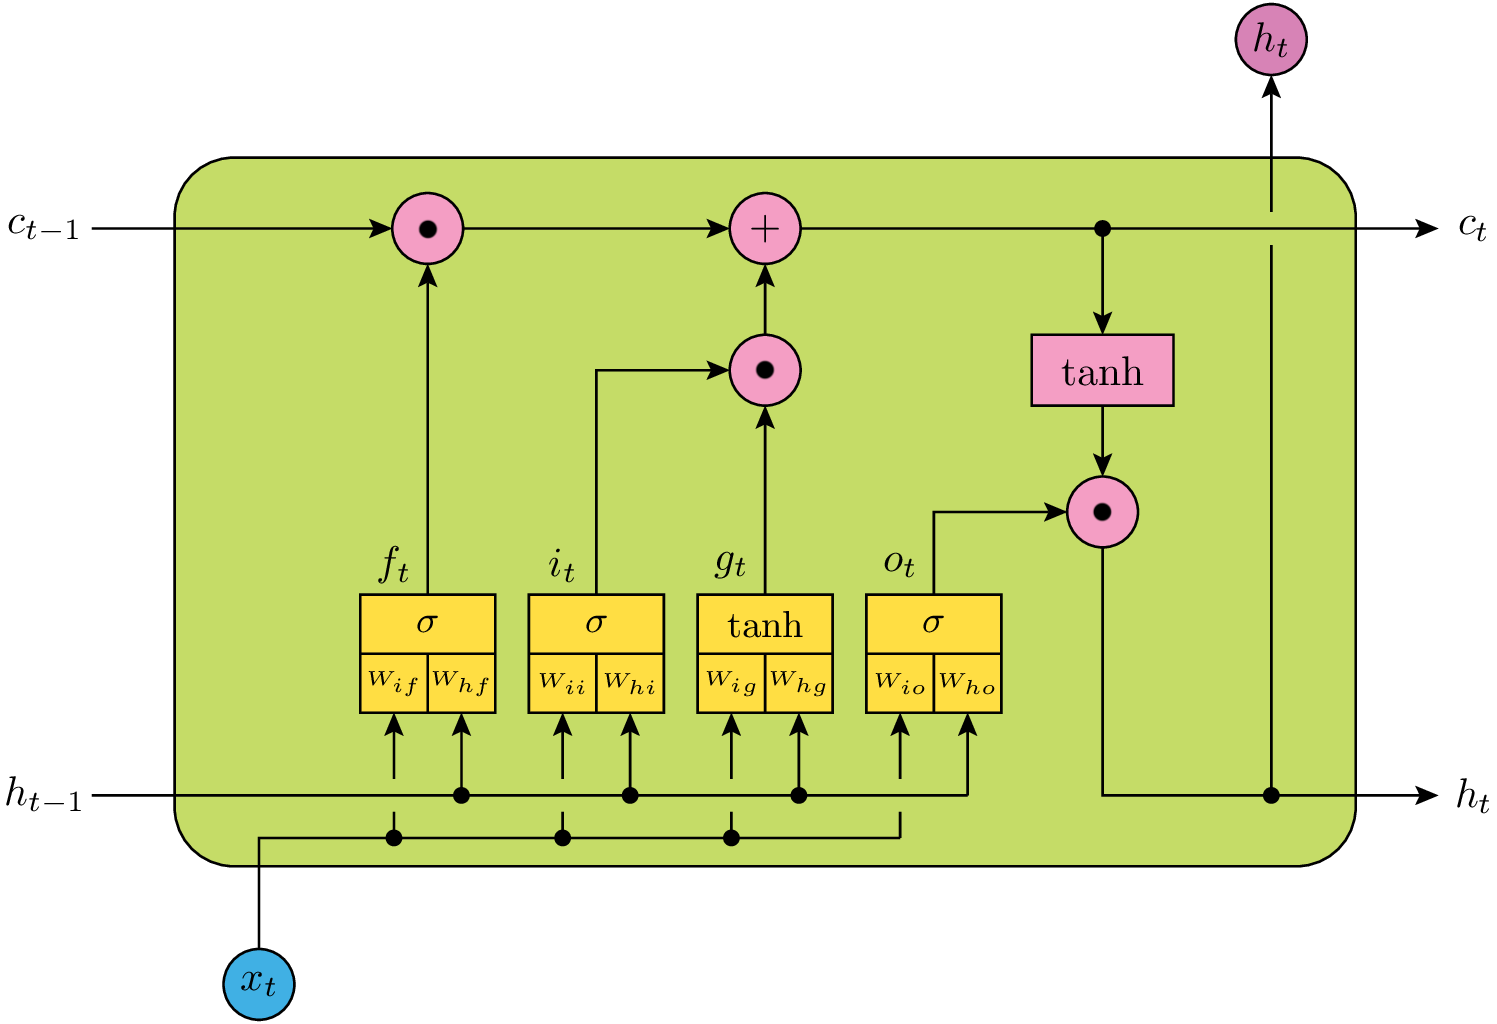
\includegraphics[width=10cm]{lstm_cell.png}
    \caption{LSTM cell \cite{lstmcell_img}}
    \label{fig:lstmCell}
\end{figure}
%=======================================================================================================================
\subsection{Graph Neural Networks}
Graphs are commonly used to describe and analyze entities with relations or interactions. Still, today's deep learning modern toolbox is specialized for simple data types, e.g., grids for images, sequences for text or speech. These data structures have spatial locality, the grid size or sequence length is fixed and can be resized. We can also determine the starting position and ending position. Graph problems are, on the other hand, much more challenging to process as they have arbitrary size and complex topological structure (i.e., no spatial locality like grids). Graphs also have no fixed node ordering or reference point compared to grids or sequences. For such Franco Scarselli et al. introduced graph neural network (GNN) \cite{graph}.

GNN is designed similarly to CNN. As previously noted, CNN operates on images. Given an image, a rectangular grid, the convolutional layer takes a subpart of the image, applies a function to it, and produces a new part, a new pixel. This is iterated for the whole image. What actually happened is the new pixel resulted in aggregated information from neighbors and itself. This cannot be easily applied to graphs as they have no spatial locality and no fixed node ordering. As implied, a GNN design stands on passing and aggregating information from neighbors. 

\subsubsection{Node embedding}

Graphs require a concept called node embedding. The general idea is to map nodes to a lower dimensional embedding space, where similar nodes in the embedding space approximate similarity in the graph network. For example, we can map a 3D vector to a 2D vector. Node embedding is useful for learning node representations and similarities and can be trained on graphs with arbitrary structures.

Nodes have embeddings at each layer. Taken node $v$, its layer-0 embedding would be its feature vector $x_v$. If we want layer-1 embedding, we will explore node $v$'s neighbors. These neighbors are so-called one hop away from our original vector $v$. We take the feature vector of these nodes and aggregate the information into one single $x_v$ feature vector. Layer-k would get information from nodes that are k hops away. 

\begin{figure}[h]
  \centering
  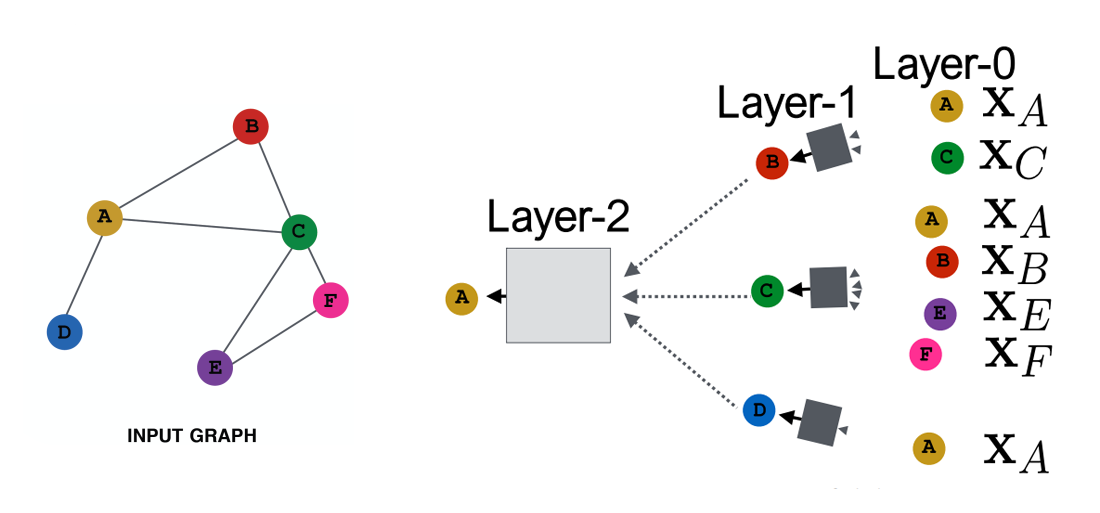
\includegraphics[width=12cm]{gnn_layers.png}
  \caption{Layer-2 embedding applied on node $A$ aggregating infromation from its neighborhood \cite{stanford}}
  \label{fig:gnn_layers}
\end{figure}

The described process is called neighborhood aggregation. If we want to predict node $v$, we need information from its neighborhood, meaning we need a way to propagate the message. Messages are passed and transformed through edges. All received messages are aggregated into a new message and then passed on. This is done systematically for every node in the graph.

The aggregation itself is done by a neural network. This implies the key difference from a typical ANN. Every node gets to define its own neural network and GNN is defined by multiple neural networks.

\begin{figure}[h]
  \centering
  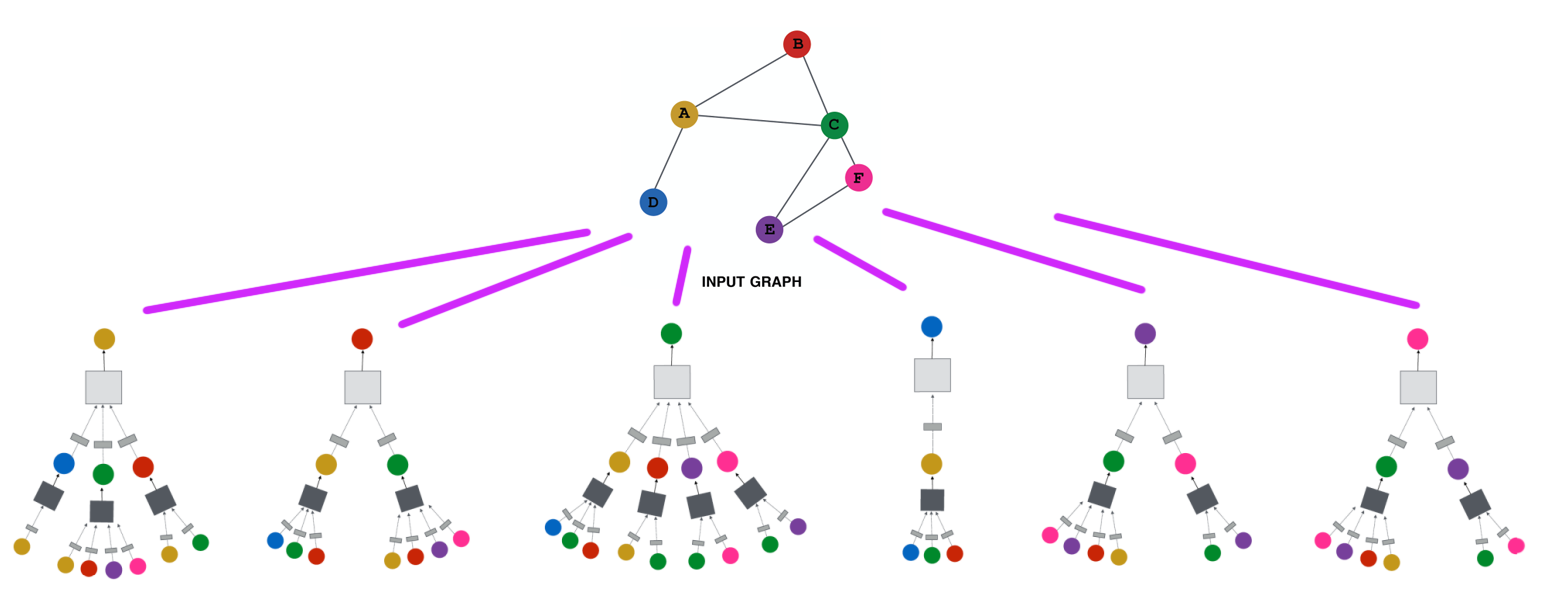
\includegraphics[width=12cm]{gnn_graph.png}
  \caption{Neural network of each node for given input node graph \cite{stanford}}
  \label{fig:gnn_graph}
\end{figure}

Using a neural network for each node in the graph, we generate a low-dimensional vector representation, embedding. The network optimizes its parameters to capture important information about the node graphs. The optimization is typically done by minimizing a loss function expressing dissimilarity between predicted and targeted node embeddings. Similar nodes are close to each other, whereas dissimilar are embedded far apart. 

\subsubsection{Geometric graphs}
TODO SECTION
Geometric graph is a graph where its nodes represent coordinates in d-dimensional space. Invariant to translation, rotation and scale

... todo more mat... 

%=======================================================================================================================
%=======================================================================================================================\newpage\cleardoublepage
	%========================================================================================================
	\setsecnumdepth{all}
	\chapter{Polygon Mesh}\label{ch:polygon_mesh}
	
In the following chapter, we will discuss shape representation in computer graphics. Explore some of their properties and what tools can be used to modify them. Some of the usual data structures to represent a geometric shape and position within a 3D space are:

\begin{itemize}
    \item \textbf{Mesh} is a set of vertices, edges, and faces defining a 3D object. It is especially used in computer graphics, and it is a simple way to represent complex 3D shapes. A face is a polygon with a minimum of 3 vertices. The most commonly used is a triangle. If a face is made of 4 vertices, it is called a quad, and more than four is called a general polygon. In our case, when we mention faces, we will have triangles in mind. These faces then form a general surface. 
    \begin{figure}[h]
        \centering
        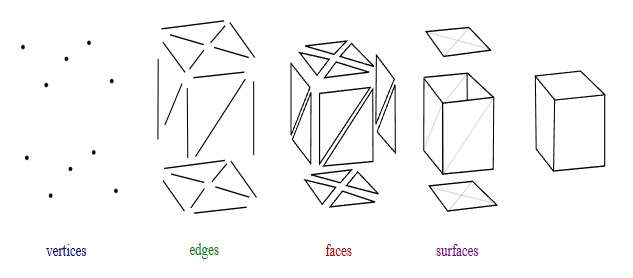
\includegraphics[width=11cm]{mesh.png}
        \caption{Elements of mesh object \cite{stanford}}
        \label{fig:mesh}
    \end{figure}
    
    A 3D object can have a color. To do so, we assign color values to every vertex of the 3D object. The pixel color of the triangle is determined based on the three vertices by which it is made.
    
    \begin{figure}[h]
        \centering
        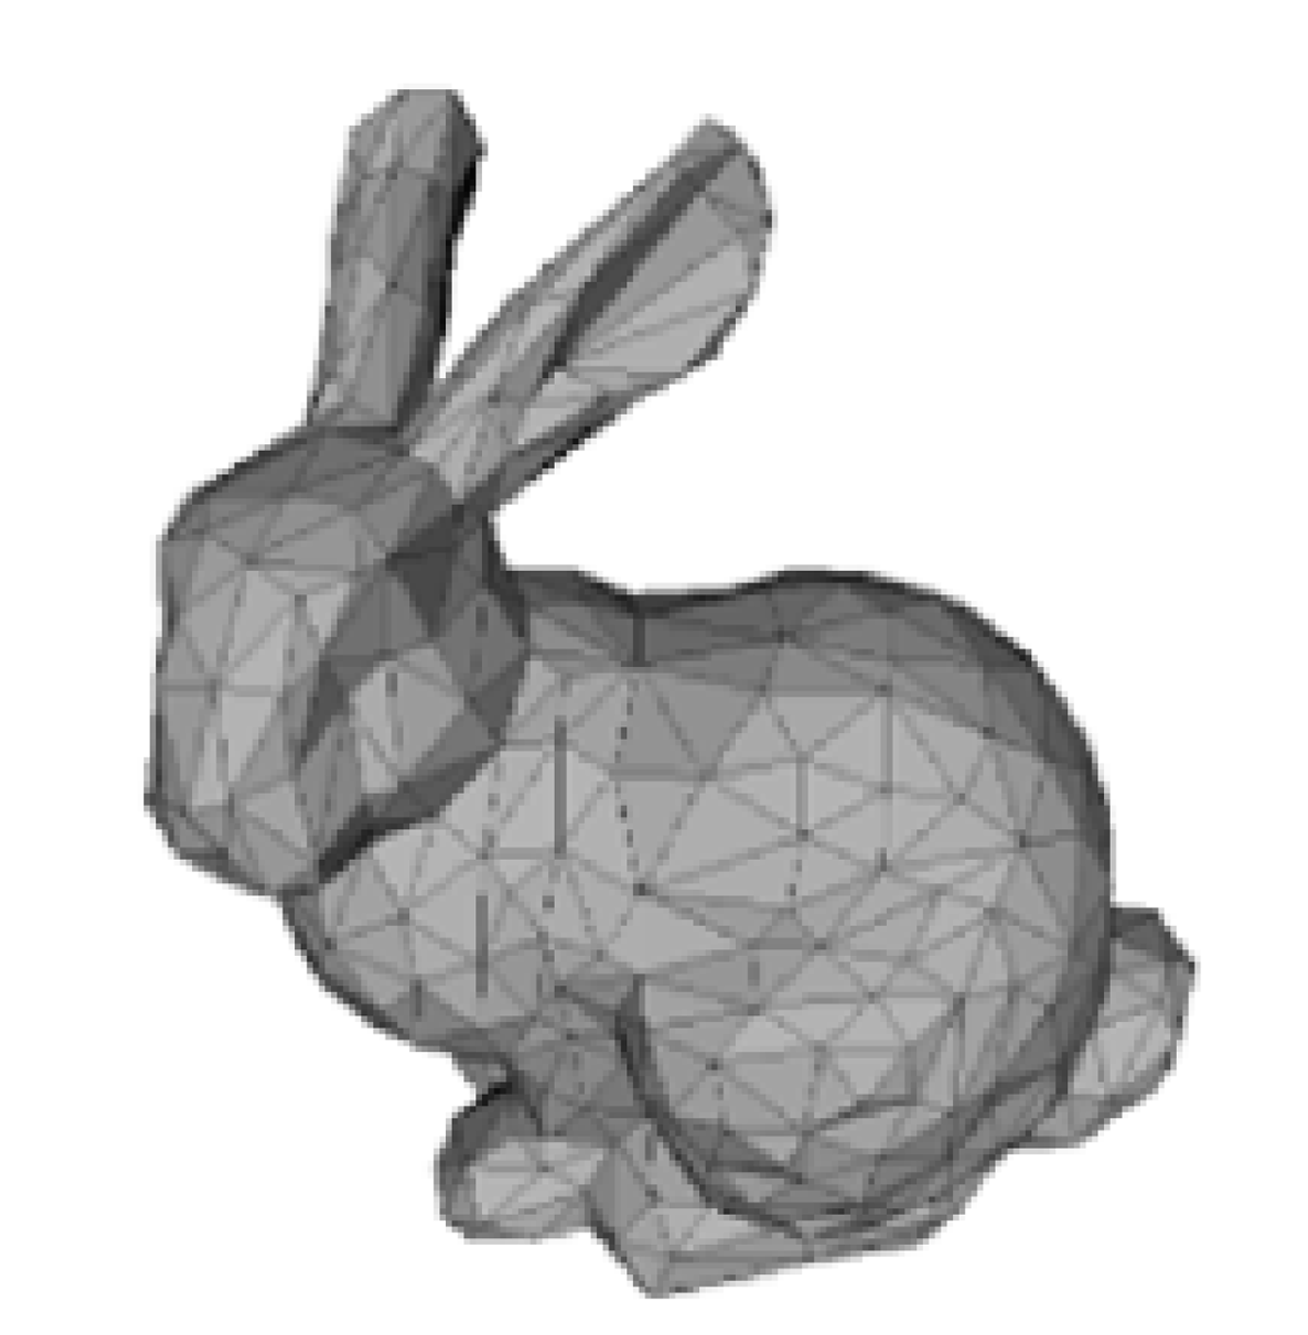
\includegraphics[width=4cm]{rabbit_mesh.png}
        \caption{Stanford bunny model made of mesh \cite{stanford}}
        \label{fig:rabbit_mesh}
    \end{figure} 

    \item \textbf{Voxel} objects are in comparison with mesh objects solid. As already said, mesh objects are created from a surface of little triangles, but it is also worth noting that this object is hollow, just like a ballooon. On the other hand, if a model is created from voxels, abbreviation from volumetric pixels, it means that the object was created from cubes and the object itself is solid, its inside also holds information. The working scene is a 3D grid, and its data point holds information about opacity, color, and material information is often also stored.
    
    \begin{figure}[h]
        \centering
        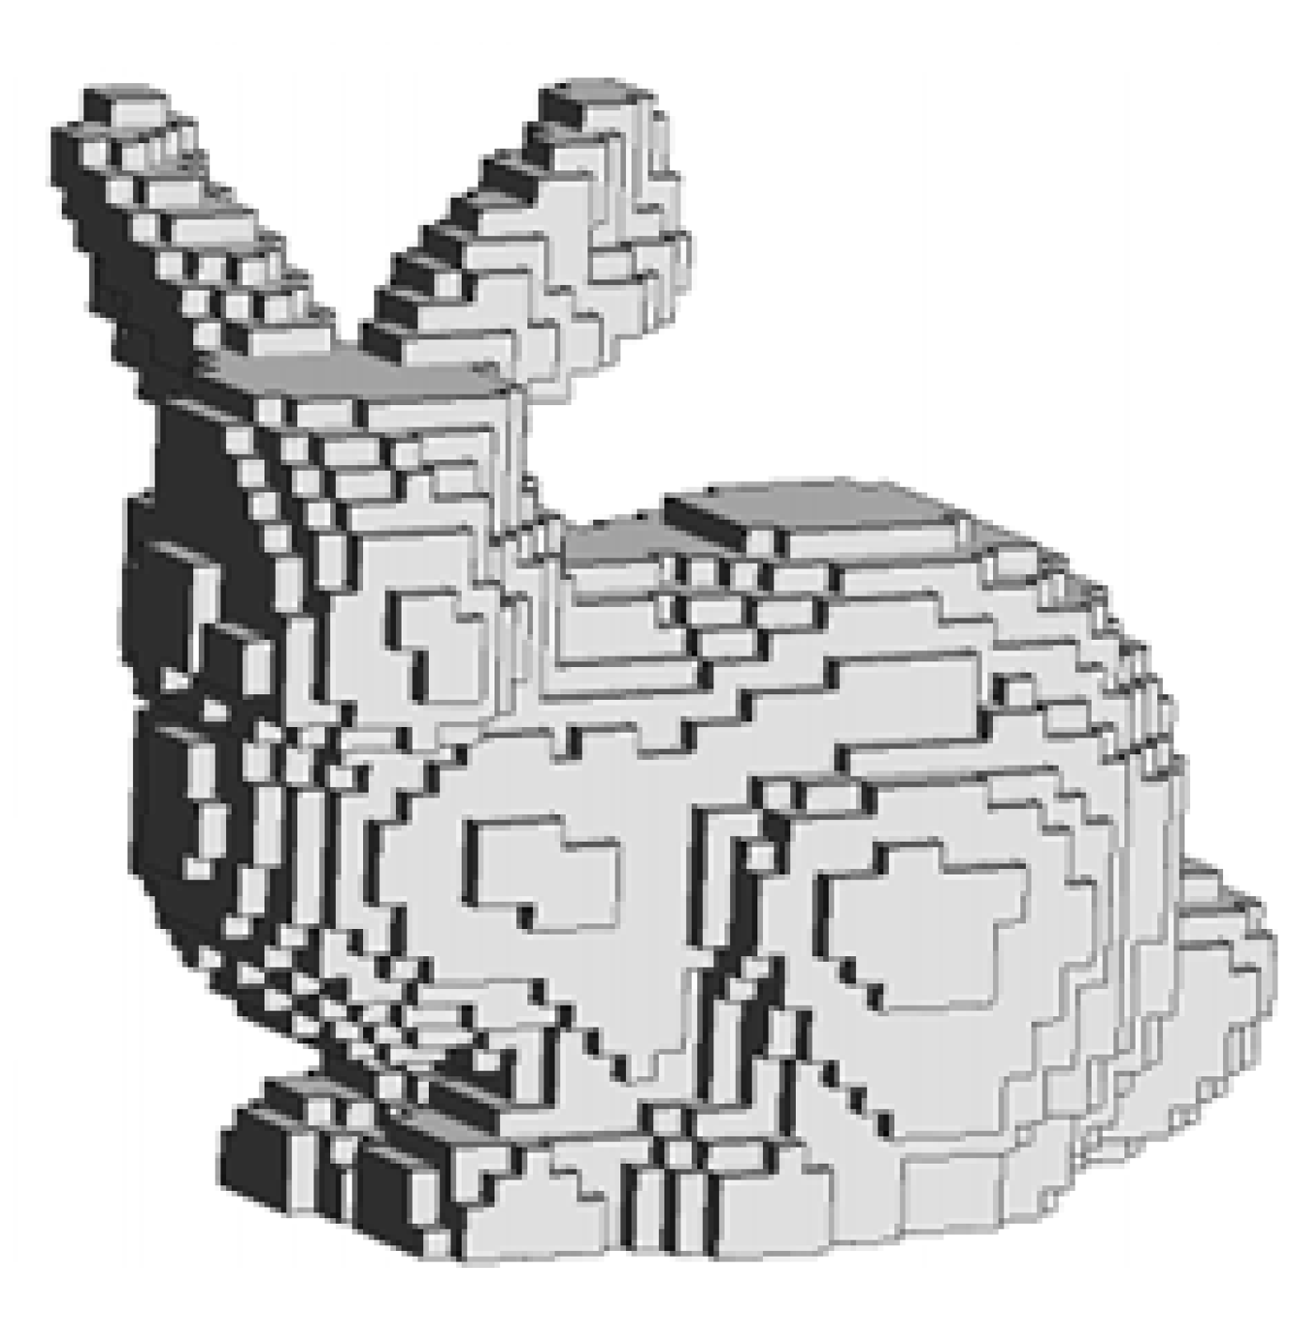
\includegraphics[width=4cm]{rabbit_voxel.png}
        \caption{Stanford bunny model made of voxels \cite{lstmcell_img}}
        \label{fig:rabbit_voxel}
    \end{figure}

    Voxels are often used in medicine and terrain representation. Voxel terrain can represent overhangs, caves, arches, and other, which is difficult to represent using heightmaps, which represents only top-layer data, and anything below it would be filled with no option for holes.

    The main disadvantage of voxels is the resolution. If we want to have a highly detailed voxel model, we would have to increase the resolution of the whole scene.

    \item \textbf{Point cloud} is a collection of points plotted in 3D space. Each point contains position coordinates, color values, and luminance values, determining how bright a point is.
    
    Points are usually acquired by a 3D scanner or photogrammetry software. Scanners work by sending out pulses of light to the object and measuring how long each point takes to reflect back and hit the scanner. These measurements are used to determine the exact positions of points on the object, creating a point cloud. Photogrammetry is a process to create measurements from pictures. It uses photos of an object to triangulate points on the object and plot these points to 3D points, resulting in point clouds.
    
    \begin{figure}[h]
        \centering
        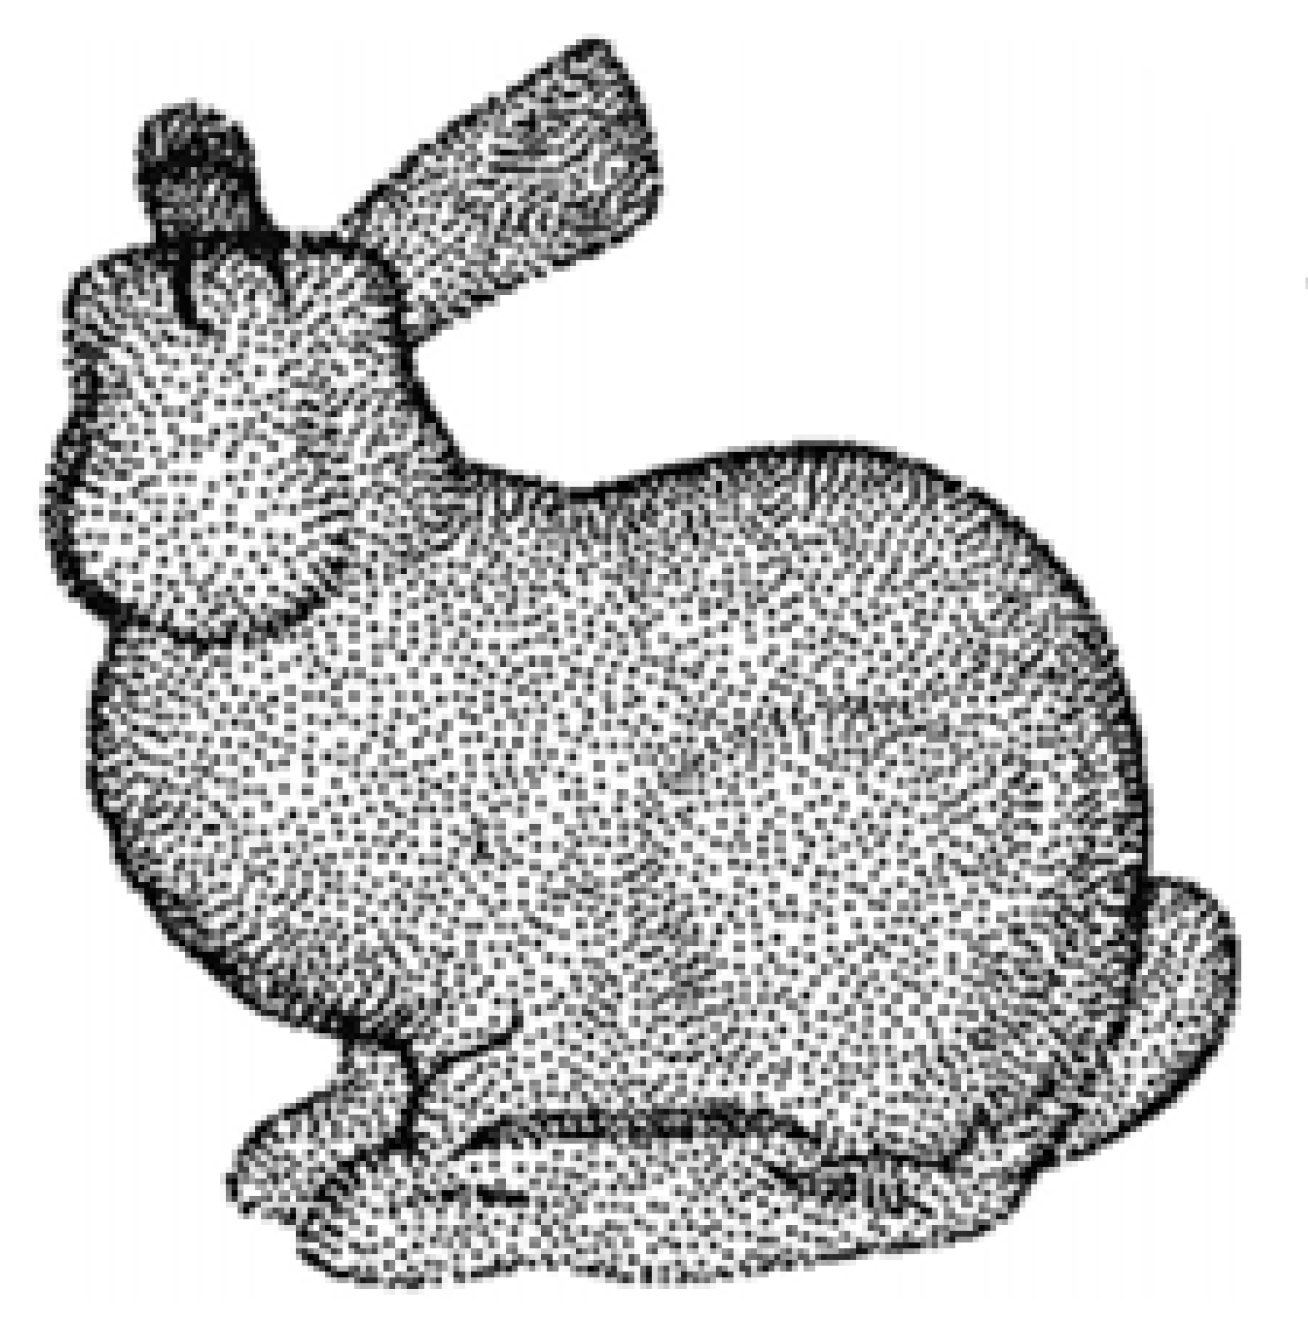
\includegraphics[width=4cm]{rabbit_cloud.png}
        \caption{Stanford bunny model made of point clouds \cite{stnaford}}
        \label{fig:rabbit_cloud}
    \end{figure}
  \end{itemize}

  In terms of the thesis and its goal, we will mainly explore mesh polygons and their edge flow properties while also exploring polygon reduction operations on them.

\section{Edge flow}

Edge flow is a fundamental concept in 3D modeling. The general goal is to ensure that mesh edges follow the curves of an object. A mesh with distinctly different edge flows can represent the same object while preserving the same shape. The key difference and significance of edge flows plays in the world of animation, overall any deformation operation performed on the object. In general, a good edge flow has uniformly distributed points along the 3d model, meaning the length and the area of each primitive is also of similar if not equal sizes. 

\begin{figure}[h]
    \centering
    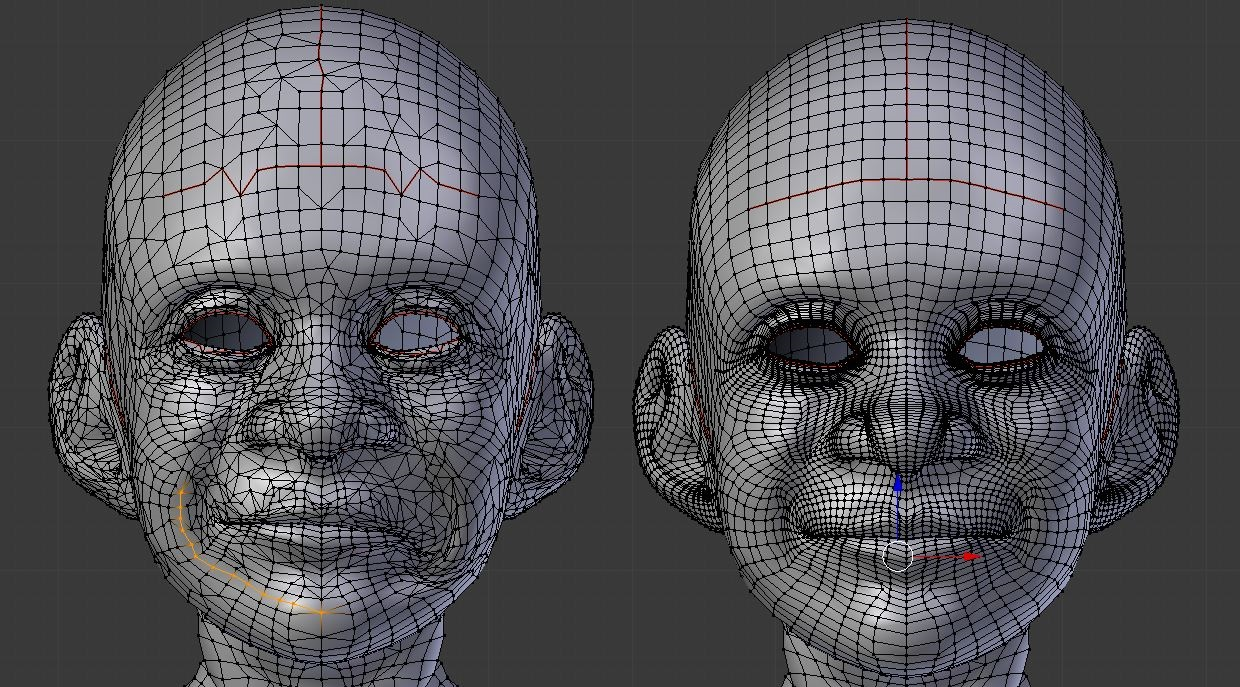
\includegraphics[width=12cm]{topology.png}
    \caption{A mesh object constructed with 2 different edge flows \cite{decimation}}
    \label{fig:topology_comp}
\end{figure}

An optimal edge flow allows smooth and natural deformations. In the case of figure \ref{fig:topology_comp}, if we want to animate various facial expressions, the left example would have distorted wrinkles. In contrast, the right example would allow for natural mimicry, as we are familiar with in real life. A more expressive example would be in \ref{fig:planar_def}, where we can see a plane of two different topologies having different behavior if bent. The left example has slight bumpy artifacts, while the right preserves smooth surface transition.

\begin{figure}[h]
    \centering
    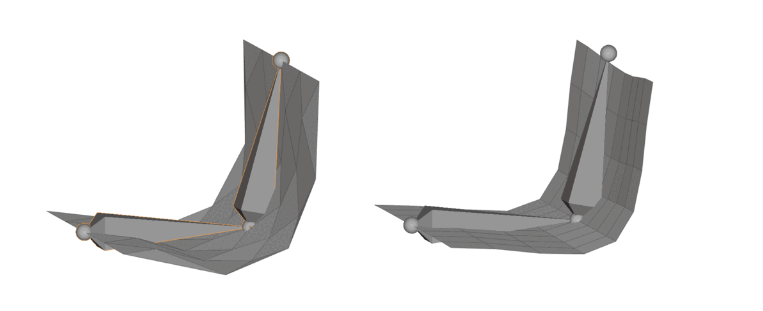
\includegraphics[width=12cm]{planar_deform.png}
    \caption{Deformation of the same object with different edge flow \cite{topology_animation}}
    \label{fig:planar_def}
\end{figure}

Edge flows are manually crafted by 3D artist and require experience to reach their optimal form. They are either being considered from the beginning while creating the 3D mesh or as a post-correction, where the acquired 3D mesh does not meet the required quality needed for future work. One of the possible reasons for having insufficient quality could be caused by polygon reduction.

\section{Polygon reduction}
Polygon reduction is a common practice for performance and memory optimization as a higher number of polygons may introduce greater details, but they also bring high demand on hardware requirements. A high polygon mesh is usually a byproduct of the 3D scanning process where the resulting 3D mesh can be of enormous memory size. Most importantly, the reduced amount should be considered as the reduction can lose the visual representation of the object and its key features. The general goal is to balance visual quality and performance optimization. Following, we will list some of the most used techniques for polygon reduction and their effect on the resulting edge flow. Edge flow is a fundamental concept in 3D modeling, playing a pivotal role in natural 3D model deformations mostly used in animation. 

\section{Decimation}

Decimation is a commonly used method for quick polygon reduction. It reduces the percentage of vertices and edges uniformly while preserving the overall shape of the reduced object, but it does not handle fine details well. Most 3d modeling software, such as Blender, Maya, 3ds Max, Zbrush, and Cinema4D, support decimation since it is a common technique. The overall control or workflow may differ, but the general concept remains the same.\cite{decimation}

\begin{figure}[h]
    \centering
    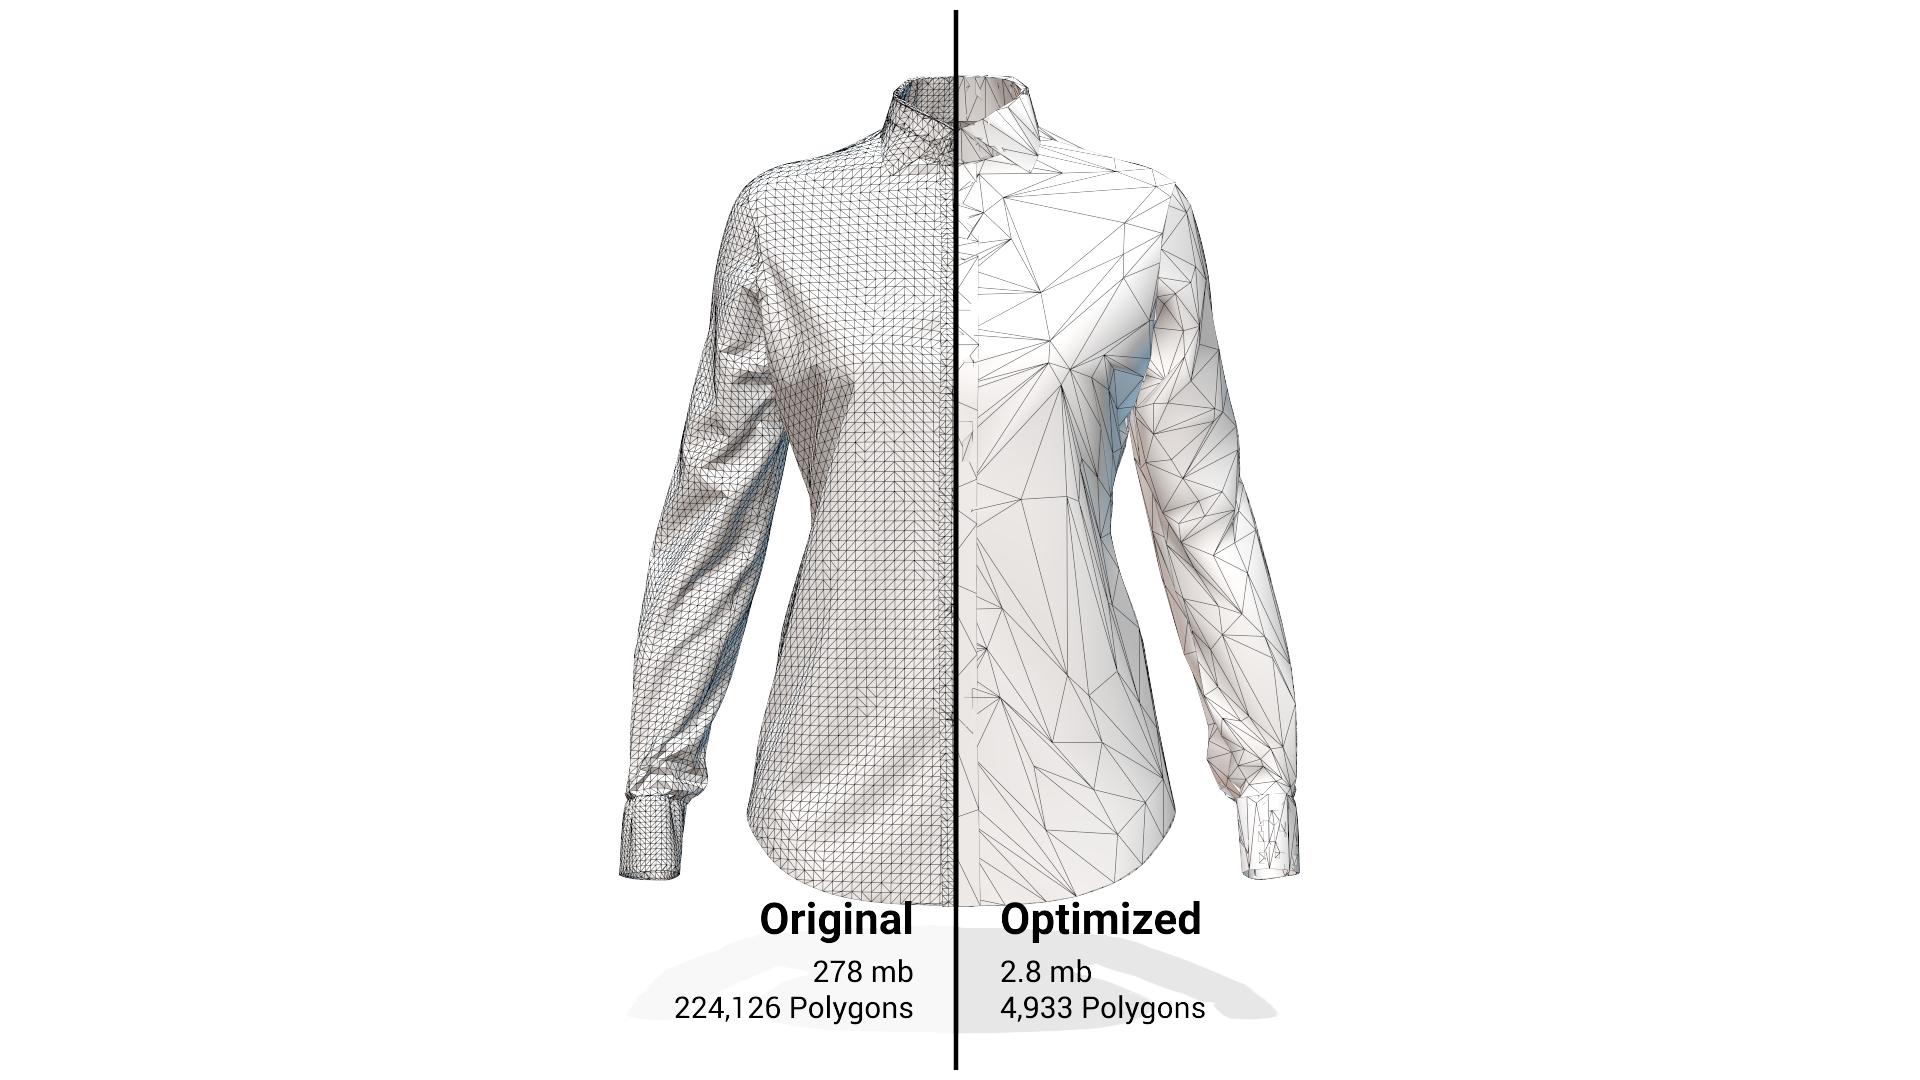
\includegraphics[width=12cm]{ShirtComparison.png}
    \caption{Decimation applied on shirt 3D mesh \cite{decimation}}
    \label{fig:shirt_comp}
\end{figure}

As seen in \ref{fig:shirt_comp}, the optimized 3D mesh may be optimized in the number of polygons, but its edge flow suffered greatly. If the shirt was part of any animated object, its part would deform unnaturally in undesired ways.

\section{Retopology}

Retopology is a semi-automatic method requiring high user input. Retopology requires a user to manually outline the required surface by hand while hinting at its edge flow by following the model's edges before the 3D software follows the outlines and draws a polygon. This gives a user high control over its model but is highly demanding on general experience and skill while identifying the edges. From a quality perspective, the resulting model will be suitable for animations and smooth 3D model deformations. Still, from a workflow efficiency standpoint, producing one of these reduced models requires a lot of time.

\begin{figure}[h]
    \centering
    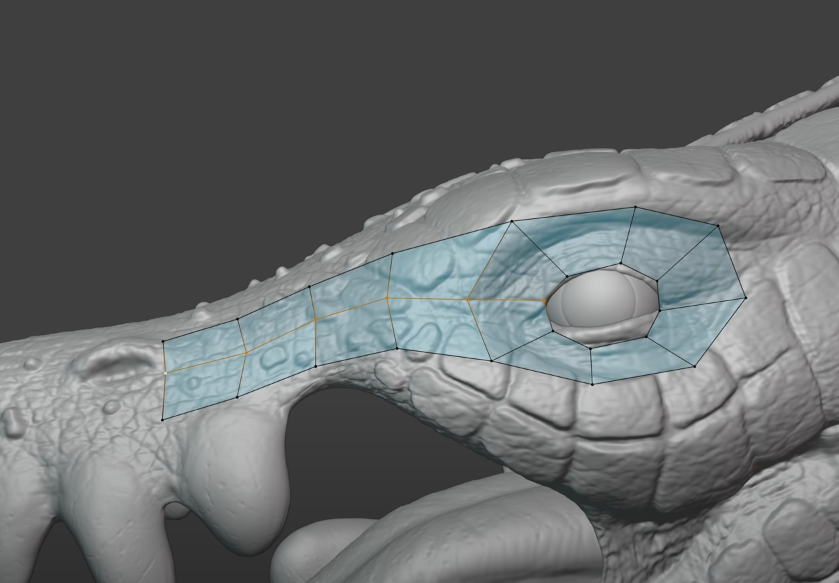
\includegraphics[width=12cm]{retopology.png}
    \caption{Retopology surface manually created lizard 3D mesh \cite{retopology}}
    \label{fig:retopology}
\end{figure}

\section{Quad Remeshing}

Instant remesh

Eh...

Decimation -> automatic reduction
Decimation does not preserve edge flow

* polygon reduction tools
* retopology -> requires manual work Blender
* quad remeshing -> often use to preserve nice deformation -> for animation -> main nemesis
* edge collapse -> manual work

These reduction techniques don't ensure so called edge flow, a fundamental concept in 3D modeling playing a pivotal role in natural 3D model deformation mostly used in animation.\newpage\cleardoublepage
	%========================================================================================================
	\setsecnumdepth{all}
	\chapter{Related Work}\label{ch:related_works}
	The main challenge is that there is currently no way to express an optimality of an edge flow by one number, which is critical for learning methods when we want to compute a loss function. We previously mentioned that an optimal flow has uniformly distributed points, edge lenghts and overall area of a primitive. One way to possibly achieve that is to look at the task at hand from different perspective. Instead of doing a correction of the given 3D mesh, we will try to reconstruct the shape of a given 3D mesh with better topology.

In this chapter we will explore researches using neural networks for 3D mesh reconstruction. 

\section{Retrieve and deform a template}

Retrieve and deform a template is a two step solution. First a most suitable template is picked and then it is deformed to the target object. The input is processed with neural network which classifies which template is best suited, such as BCNet \cite{bcnet}, MultiGarment Net\cite{mgn} or ShapeFlow \cite{shapeflow}. As seen in Figure \ref{fig:bcnet} and \ref{fig:shapeflow}, a nearest-neighbor template is retrieved from the embedded space and then a deformation network is applied.

\begin{figure}[h]
    \centering
    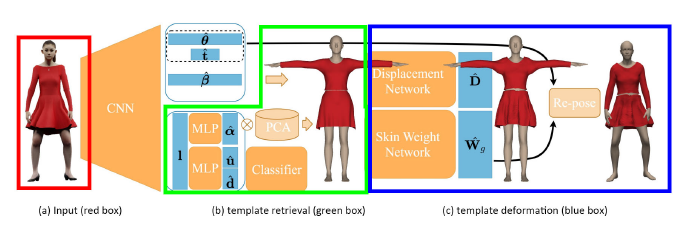
\includegraphics[width=12cm]{bcnet.png}
    \caption{Overview of retrieve and deform shape reconstruction using BCNet \cite{bcnet}}
    \label{fig:bcnet}
\end{figure}

\begin{figure}[h]
    \centering
    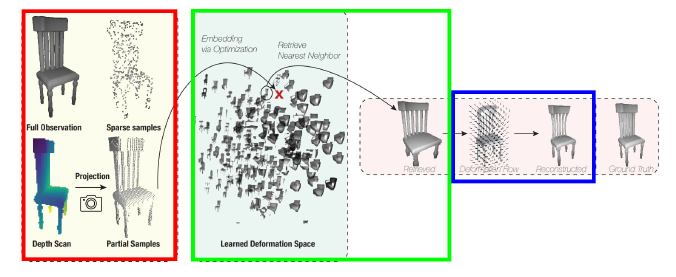
\includegraphics[width=12cm]{shapeflow.png}
    \caption{Overview of retrieve and deform shape reconstruction using ShapeFlow \cite{shapeflow}}
    \label{fig:shapeflow}
\end{figure}

\section{Deform a primitive}

Retrieve and deform solution expects a high quality templates and they were also highly specialized in certain category type, which makes the overall input and output then highly specialized. Other method often used for aproximating to target object from a single image would be deforming a primitive. Popular representation in Pixel2Mesh \cite{p2m}, Pixel2Mesh++ \cite{p2mpp}, Neural mesh flow \cite{neuralFlow} was a simple sphere. 

Pixel2Mesh had a 2D CNN extracting features from a single image which is then leveraged by a deformation block, progressively deforming a sphere into the desired 3D model. The cascaded mesh deformation network is a graph-based convolution network, containing three deformation blocks intersected by two graph unpooling layers, which increases the number of vertices. With given face the points were added to the middle of each connecting edges. Connecting these newly added points then forms a new set of primitive faces, while also ensuring even distribution of vertices and their degrees. The improved Pixel2Mesh is extracts features from multiple view images, increasing the reconstruction accurancy. 

\begin{figure}[h]
    \centering
    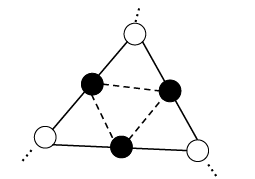
\includegraphics[width=6cm]{p2m_unpooling.png}
    \caption{Graph unpooling\cite{p2m}}
    \label{fig:p2munpooling}
\end{figure}

\begin{figure}[h]
    \centering
    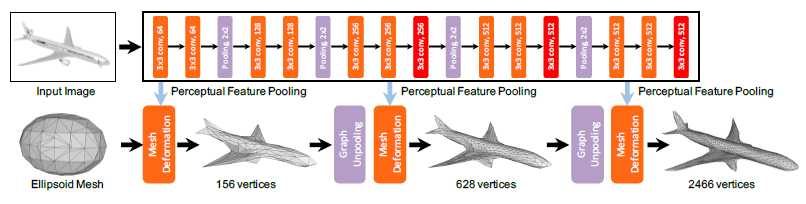
\includegraphics[width=12cm]{p2m.png}
    \caption{Pixel2Mesh architecture overview \cite{p2m}}
    \label{fig:p2m}
\end{figure}

The Neural mesh flow shares very similar architecture as Pixel2Mesh in using three deform blocks.

Neural Mesh Flow (NFM) as seen in Figure \ref{fig:netflow}, learns to auto-encode 3D shapes. NMF broadly consists of four components. First, the target shape is encoded by uniformly sampling N points from its surface and feeding them to a PointNet \cite{pointnet} encoder to get the global shape embedding. Second, NODE blocks diffeomorphically flow the vertices of template sphere towards target shape conditioned on shape embedding. Third, the instance normalization layer performs non-uniform scaling of NODE output to ease cross-category training. Finally, refinement flows provide gradual improvement in quality.

\begin{figure}[h]
    \centering
    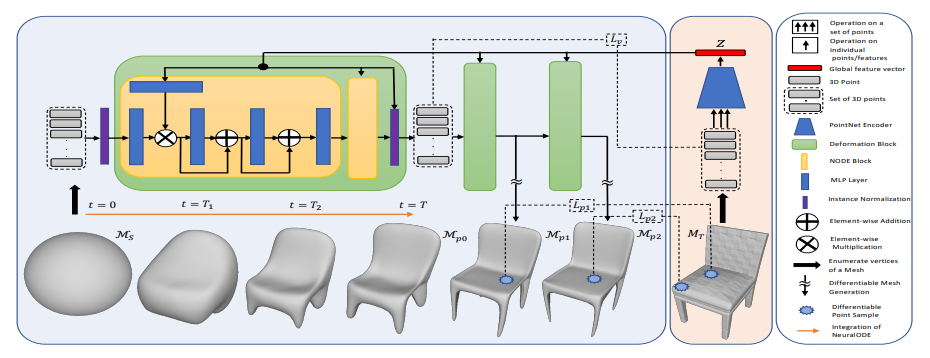
\includegraphics[width=12cm]{netflow.png}
    \caption{Neural Mesh flow architecture overview \cite{neuralFlow}}
    \label{fig:netflow}
\end{figure}




The mesh reconstruction is often done from voxels, point clouds, single images, and multi-view images, respectively. There was previously no real purpose of doing a reconstruction from a mesh as in our case.

universal solution, depends on previous topology quality\newpage\cleardoublepage
	%========================================================================================================
	\setsecnumdepth{all}
	\chapter{Implementation}\label{ch:implementation}
	\input{chapters/implementation.tex}\newpage\cleardoublepage
	%========================================================================================================
	\setsecnumdepth{all}
	\chapter{Experiments}\label{ch:experiments}
	\input{chapters/experiments.tex}\newpage\cleardoublepage
	%========================================================================================================
	\setsecnumdepth{all}
	\chapter{Conclusion}\label{ch:conclusion}
	\input{chapters/conclusion.tex}\newpage\cleardoublepage


\bibliographystyle{iso690}
\bibliography{mybibliographyfile}

\setsecnumdepth{all}
\appendix

\chapter{Acronyms}
% \printglossaries
\begin{description}
	\item[ANN] Artificial Neural Network
	\item[RNN] Recurrent Neural Network
	\item[CNN] Convolutional Neural Network
	\item[LSTM] Long Short-Term Memory
	\item[ReLU] Rectified Linear Unit
\end{description}


\chapter{Contents of enclosed CD}

%change appropriately

\begin{figure}
	\dirtree{%
		.1 README.md\DTcomment{the Markdown file with description}.
		.1 executables\DTcomment{the directory with executables}.
		.2 Dataset\DTcomment{the directory of the original dataset}.
		.2 TrainedModel\DTcomment{the directory of trained model}.
		.2 DataSampler.exe\DTcomment{data sampling application}.
		.2 model\_trainig.py\DTcomment{model training Python script}.
		.2 GestureApp.exe\DTcomment{gesture recognition demo application}.
		.1 src\DTcomment{the directory of source codes}.
		.1 text\DTcomment{the directory of \LaTeX{} source codes of the thesis}.
		.1 environment.yml\DTcomment{configuration file for conda environment}.
		.1 BP\_Viet\_Anh\_Tran\_2021.pdf\DTcomment{the thesis text in PDF format}.
	}
\end{figure}



\end{document}
